\documentclass{article}
\usepackage[spanish]{babel}   
\usepackage[numbers,sort&compress]{natbib}
\usepackage{float}
\usepackage{listings}
\usepackage{graphicx} 	% Nos permite importar imagenes 
\usepackage{subfigure}
\usepackage[left=3cm,right=3cm,top=3cm,bottom=3cm]{geometry}

%-------------------------- Por si se romple la URL --------------------------
\usepackage[hyphens]{url}
\usepackage[hidelinks]{hyperref}
\hypersetup{breaklinks=true}	
\urlstyle{same}
\usepackage{cite}
%-------------------------- Por si se romple la URL --------------------------

\title{Reporte Tarea 11}
\author{Victor Alejandro Oviedo Martínez}



\begin{document}
\maketitle
\hrule

\section{Introduccón}\label{intro}
Para esta onceava tarea \citep{DRA.P11} se ha estudiado el tema frentes de Pareto, el cual tiene la capacidad de encontrar soluciones en problemas de optimización múlticriterio. Esto quiere decir que a un problema con múltiples objetivos, en donde  estos objetivos pueden contraponerse, mientras uno mejora los otros empeoran y viceversa, el objetivos es encontrar el subconjunto de soluciones que mejor resultado tengan promediando sus objetivos.\\




\section{Desarrollo}

Para esta onceava tarea se ha planteado el siguiente problema: Grafica el porcentaje de soluciones de Pareto (ojo, no es lo mismo que se grafica en el código ejemplo) como función del número de funciones objetivo para 
$k \in [2,12]$ con diagramas de violín combinados con diagramas de caja-bigote, verificando que diferencias observadas, cuando las haya, sean estadísticamente significativas. Razona en escrito a qué se debe el comportamiento observado.\\


Para el desarrollo de esta tarea se a utilizado el código ejemplo proporcionado por \citet{DRA.Code}, el cual tiene el objetivo de desarrollar una simulación para encontrar el frente de Pareto dependiendo los objetivos (\texttt{k}) que se quieran simular.\\  

Iniciando la edición del código \citep{DRA.Code}, se ha agregado la función \texttt{porcentaje(f,total)} con el fin de calcular el porcentaje del frente de Pareto obtenido, ademas se ha convertido en función la mayor parte del código base con el fin  de repetir este proceso con mayor facilidad. A esta nueva función lleva por nombre: \texttt{simu(k)}, y cómo se puede observar solo será necesario especificar los objetivos a generar. Una vez generada la nueva función, se utilizan ciclos \texttt{for} para realizar cuarenta repeticiones de cada objetivo. Por lo tanto, al final tendremos 440 datos con los porcentajes de soluciones de Pareto en la variable \texttt{POR} que posterior mente se graficarán.

\begin{lstlisting}[language=Python]
rep = 40
POR = []
for k in range(2,13):
    for i in range(rep):
        print("----",k,",",i,"----")
        s = simu(k)
        POR.append(s)
\end{lstlisting}






\section{Conclusión}

En la figura \ref{f1} se puede observar los resultados de la simulación. 

\begin{figure}[H]
\begin{center}
	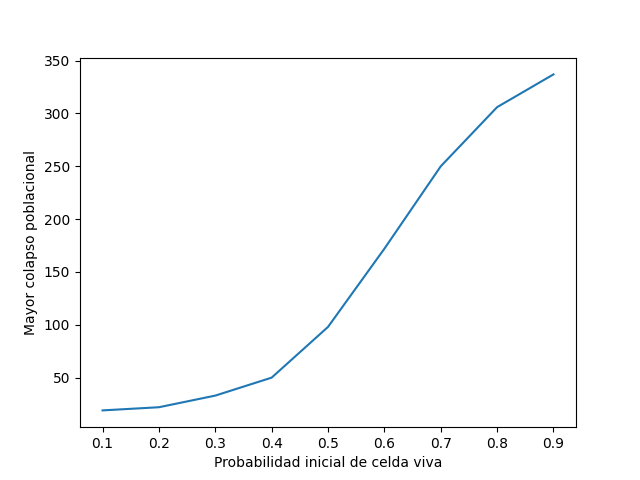
\includegraphics[height=4.in]{/Users/victor/Desktop/Figure_1.png}
	\caption{ Simulación para $k \in [2,12]$, 40 repeticiones.}
	\label{f1}
\end{center}
\end{figure}

Cómo conclusión y con base en los datos se observa como a medida que se aumentan la cantidad de objetivos (\texttt{k}) también aumenta el porcentaje de la carnalidad de Pareto con respecto al total de soluciones.
%-------------------------- Por si se rompe la URL --------------------------
\Urlmuskip=0mu plus 1mu\relax
%-------------------------- Por si se rompe la URL --------------------------
\bibliography{ref.Tarea11.bib}
\bibliographystyle{plainnat}

\end{document}